% answers.tex —— 1996 年·上海卷·文史类 · 参考答案与详细解析片段
% 由 tools/generate_projects.py 依来源总账自 1996/1996_数学真题_上海文史_试题.md + 1996/1996_数学真题_上海文史_解析正文.md + 1996/1996_数学真题_上海文史_答案要点.md 生成，勿手改（改源 MD 后重跑）


\begin{gknotice}
\textbf{解析归属}：下列第 19—24 题推导依据固定来源 PDF 第 5—8 页（印刷页码 87—90）逐步转录、排版；第 1—18 题在固定来源中只有答案键，没有逐题推导，故如实标明未载解析，不在本源文件补造独立解法。来源出版者与官方性尚未核实；本文件不是独立盲核或正式数学验收结论。
\end{gknotice}

\begin{answer}
\gksolhead{1}{}

\textbf{题目}：

\Needspace{5\baselineskip}
已知集合

\nopagebreak[4]
\[
M=\{(x,y)\mid x+y=2\},\qquad N=\{(x,y)\mid x-y=4\},
\]

那么集合 $M\cap N$ 为\mbox{（　　）}。

（A）$x=3,\ y=-1$　　（B）$(3,-1)$　　（C）$\{3,-1\}$　　（D）$\{(3,-1)\}$

\Needspace{4\baselineskip}
\textbf{解析}

固定来源第 5 页仅列本题答案为 D，未载推导。这里不补写为来源解析。

\gkanswer{答案：D}

\end{answer}
\begin{answer}
\gksolhead{2}{}

\textbf{题目}：

在下列各区间中，函数 $y=\sin\left(x+\dfrac{\pi}{4}\right)$ 的单调递增区间是\mbox{（　　）}。

（A）$\left[\dfrac{\pi}{2},\pi\right]$　　（B）$\left[0,\dfrac{\pi}{4}\right]$　　（C）$[-\pi,0]$　　（D）$\left[\dfrac{\pi}{4},\dfrac{\pi}{2}\right]$

\Needspace{4\baselineskip}
\textbf{解析}

固定来源第 5 页仅列本题答案为 B，未载推导。这里不补写为来源解析。

\gkanswer{答案：B}

\end{answer}
\begin{answer}
\gksolhead{3}{}

\textbf{题目}：

过点 $(4,0)$ 和点 $(0,3)$ 的直线的倾斜角为\mbox{（　　）}。

（A）$\arctan\dfrac{3}{4}$　　（B）$\pi-\arctan\dfrac{3}{4}$　　（C）$\arctan\left(-\dfrac{3}{4}\right)$　　（D）$\pi-\arctan\left(-\dfrac{3}{4}\right)$

\Needspace{4\baselineskip}
\textbf{解析}

固定来源第 5 页仅列本题答案为 B，未载推导。这里不补写为来源解析。

\gkanswer{答案：B}

\end{answer}
\begin{answer}
\gksolhead{4}{}

\textbf{题目}：

在下列命题中，真命题是\mbox{（　　）}。

（A）若直线 $m,n$ 都平行于平面 $\alpha$，则 $m\parallel n$。

（B）设 $\alpha-l-\beta$ 是直二面角。若直线 $m\perp l$，则 $m\perp\beta$。

（C）若直线 $m,n$ 在平面 $\alpha$ 内的射影依次是一个点和一条直线，且 $m\perp n$，则 $n$ 在 $\alpha$ 内或 $n$ 与 $\alpha$ 平行。

（D）设 $m,n$ 是异面直线。若 $m$ 与平面 $\alpha$ 平行，则 $n$ 与 $\alpha$ 相交。

\Needspace{4\baselineskip}
\textbf{解析}

固定来源第 5 页仅列本题答案为 C，未载推导。这里不补写为来源解析。

\gkanswer{答案：C}

\end{answer}
\begin{answer}
\gksolhead{5}{}

\textbf{题目}：

\Needspace{5\baselineskip}
将椭圆

\nopagebreak[4]
\[
\dfrac{x^2}{25}+\dfrac{y^2}{9}=1
\]

绕其左焦点按逆时针方向旋转 $90^\circ$ 后所得的椭圆方程是\mbox{（　　）}。

（A）$\dfrac{(x+4)^2}{25}+\dfrac{(y-4)^2}{9}=1$　　（B）$\dfrac{(x+4)^2}{25}+\dfrac{(y+4)^2}{9}=1$

（C）$\dfrac{(x+4)^2}{9}+\dfrac{(y-4)^2}{25}=1$　　（D）$\dfrac{(x+4)^2}{9}+\dfrac{(y+4)^2}{25}=1$

\Needspace{4\baselineskip}
\textbf{解析}

固定来源第 5 页仅列本题答案为 C，未载推导。这里不补写为来源解析。

\gkanswer{答案：C}

\end{answer}
\begin{answer}
\gksolhead{6}{}

\textbf{题目}：

若 $y=f(x)$ 是定义在 $\mathbb R$ 上的函数，则 $y=f(x)$ 为奇函数的一个充要条件是\mbox{（　　）}。

（A）$f(0)=0$　　（B）对任意的 $x\in\mathbb R$，$f(x)=0$ 都成立

（C）存在某一 $x_0\in\mathbb R$，使得 $f(x_0)+f(-x_0)=0$

（D）对任意的 $x\in\mathbb R$，$f(x)+f(-x)=0$

\Needspace{4\baselineskip}
\textbf{解析}

固定来源第 5 页仅列本题答案为 D，未载推导。这里不补写为来源解析。

\gkanswer{答案：D}

\end{answer}
\begin{answer}
\gksolhead{7}{}

\textbf{题目}：

如果 $\log_a3>\log_b3>0$，那么 $a,b$ 间的关系是\mbox{（　　）}。

（A）$0<b<a<1$　　（B）$0<a<b<1$　　（C）$1<b<a$　　（D）$1<a<b$

\Needspace{4\baselineskip}
\textbf{解析}

固定来源第 5 页仅列本题答案为 D，未载推导。这里不补写为来源解析。

\gkanswer{答案：D}

\end{answer}
\begin{answer}
\gksolhead{8}{}

\textbf{题目}：

在下列图象中，二次函数 $y=ax^2+bx$ 与指数函数 $y=\left(\dfrac{b}{a}\right)^x$ 的图象只可能是\mbox{（　　）}。
\nopagebreak[4]
\begin{center}% 固定来源 PDF 印刷页 84 第 8 题四组选项图象的矢量示意重绘。
% 选项相对形状、抛物线开口/过原点关系和指数曲线过 (0,1) 按原图描绘；曲线比例仅为示意。
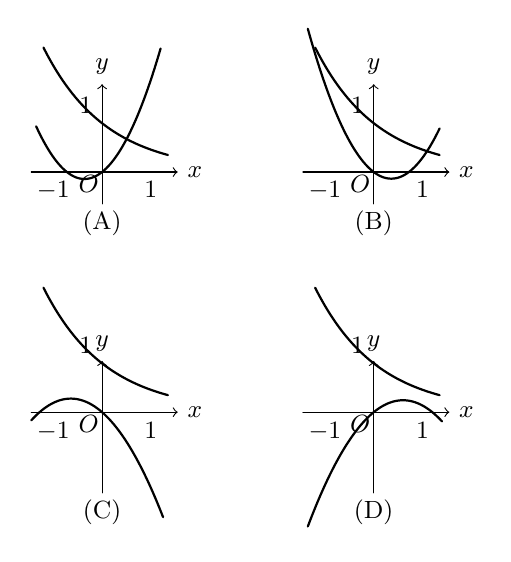
\begin{tikzpicture}[x=.62cm,y=.62cm,font=\small,line cap=round,line join=round]
  % (A) upward parabola with its second zero left of the origin.
  \begin{scope}
    \draw[->] (-1.45,0)--(1.55,0) node[right] {$x$};
    \draw[->] (0,-.65)--(0,1.8) node[above] {$y$};
    \draw[thick,domain=-1.35:1.2,samples=70,variable=\x]
      plot (\x,{1.1*\x*(\x+.72)});
    \draw[thick,domain=-1.2:1.35,samples=70,variable=\x]
      plot (\x,{exp(-.78*\x)});
    \node[below left,inner sep=1pt] at (0,0) {$O$};
    \node[below] at (-1,0) {$-1$}; \node[below] at (1,0) {$1$};
    \node[above left] at (0,1) {$1$}; \node at (0,-1.05) {(A)};
  \end{scope}
  % (B) upward parabola with its second zero right of the origin.
  \begin{scope}[xshift=3.45cm]
    \draw[->] (-1.45,0)--(1.55,0) node[right] {$x$};
    \draw[->] (0,-.65)--(0,1.8) node[above] {$y$};
    \draw[thick,domain=-1.35:1.35,samples=70,variable=\x]
      plot (\x,{1.05*\x*(\x-.72)});
    \draw[thick,domain=-1.2:1.35,samples=70,variable=\x]
      plot (\x,{exp(-.78*\x)});
    \node[below left,inner sep=1pt] at (0,0) {$O$};
    \node[below] at (-1,0) {$-1$}; \node[below] at (1,0) {$1$};
    \node[above left] at (0,1) {$1$}; \node at (0,-1.05) {(B)};
  \end{scope}
  % (C) downward parabola with its second zero left of the origin.
  \begin{scope}[yshift=-3.05cm]
    \draw[->] (-1.45,0)--(1.55,0) node[right] {$x$};
    \draw[->] (0,-1.65)--(0,1.05) node[above] {$y$};
    \draw[thick,domain=-1.45:1.25,samples=70,variable=\x]
      plot (\x,{-.68*\x*(\x+1.28)});
    \draw[thick,domain=-1.2:1.35,samples=70,variable=\x]
      plot (\x,{exp(-.78*\x)});
    \node[below left,inner sep=1pt] at (0,0) {$O$};
    \node[below] at (-1,0) {$-1$}; \node[below] at (1,0) {$1$};
    \node[above left] at (0,1) {$1$}; \node at (0,-2.05) {(C)};
  \end{scope}
  % (D) downward parabola with its second zero right of the origin.
  \begin{scope}[xshift=3.45cm,yshift=-3.05cm]
    \draw[->] (-1.45,0)--(1.55,0) node[right] {$x$};
    \draw[->] (0,-1.65)--(0,1.05) node[above] {$y$};
    \draw[thick,domain=-1.35:1.4,samples=70,variable=\x]
      plot (\x,{-.68*\x*(\x-1.2)});
    \draw[thick,domain=-1.2:1.35,samples=70,variable=\x]
      plot (\x,{exp(-.78*\x)});
    \node[below left,inner sep=1pt] at (0,0) {$O$};
    \node[below] at (-1,0) {$-1$}; \node[below] at (1,0) {$1$};
    \node[above left] at (0,1) {$1$}; \node at (0,-2.05) {(D)};
  \end{scope}
\end{tikzpicture}
\end{center}
\nopagebreak[4]
\Needspace{4\baselineskip}
\textbf{解析}

固定来源第 5 页仅列本题答案为 A，未载推导。这里不补写为来源解析。

\gkanswer{答案：A}

\end{answer}
\begin{answer}
\gksolhead{9}{}

\textbf{题目}：

\Needspace{5\baselineskip}
方程

\nopagebreak[4]
\[
\log_2(9^x-5)=\log_2(3^x-2)+2
\]

的解是 $x=\underline{\qquad\qquad}$。

\Needspace{4\baselineskip}
\textbf{解析}

固定来源第 5 页仅列本题答案为 $1$，未载推导。这里不补写为来源解析。

\gkanswer{答案：$1$}

\end{answer}
\begin{answer}
\gksolhead{10}{}

\textbf{题目}：

\Needspace{5\baselineskip}
函数

\nopagebreak[4]
\[
y=\dfrac{1}{\sqrt{\log_{1/2}(2-x)}}
\]

的定义域是 $\underline{\qquad\qquad}$。

\Needspace{4\baselineskip}
\textbf{解析}

固定来源第 5 页仅列本题答案为 $\{x\mid 1<x<2\}$（即区间 $(1,2)$），未载推导。这里不补写为来源解析。

\gkanswer{答案：$\{x\mid 1<x<2\}$}

\end{answer}
\begin{answer}
\gksolhead{11}{}

\textbf{题目}：

\Needspace{5\baselineskip}
方程

\nopagebreak[4]
\[
\sin\left(x-\dfrac{\pi}{3}\right)=\dfrac{\sqrt{2}}{2}
\]

在 $[0,\pi]$ 上的解是 $x=\underline{\qquad\qquad}$。

\Needspace{4\baselineskip}
\textbf{解析}

固定来源第 5 页仅列本题答案为 $\dfrac{7\pi}{12}$，未载推导。这里不补写为来源解析。

\gkanswer{答案：$\dfrac{7\pi}{12}$}

\end{answer}
\begin{answer}
\gksolhead{12}{}

\textbf{题目}：

函数 $y=x^{-2}\ (x<0)$ 的反函数是 $y=\underline{\qquad\qquad}$。

\Needspace{4\baselineskip}
\textbf{解析}

固定来源第 5 页仅列反函数 $y=-\sqrt{\dfrac1x}\ (x>0)$，未载推导。这里不补写为来源解析。

\gkanswer{答案：$y=-\sqrt{\dfrac1x}\ (x>0)$}

\end{answer}
\begin{answer}
\gksolhead{13}{}

\textbf{题目}：

与圆 $(x-2)^2+y^2=1$ 外切，且与 $y$ 轴相切的动圆圆心 $P$ 的轨迹方程为 $\underline{\qquad\qquad}$。

\Needspace{4\baselineskip}
\textbf{解析}

固定来源第 5 页仅列本题答案为 $y^2=6x-3$，未载推导。这里不补写为来源解析。

\gkanswer{答案：$y^2=6x-3$}

\end{answer}
\begin{answer}
\gksolhead{14}{}

\textbf{题目}：

在 $(1+x)^2(1-x)^4$ 的展开式中，$x^3$ 的系数是 $\underline{\qquad\qquad}$（结果用数值表示）。

\Needspace{4\baselineskip}
\textbf{解析}

固定来源第 5 页仅列本题答案为 $4$，未载推导。这里不补写为来源解析。

\gkanswer{答案：$4$}

\end{answer}
\begin{answer}
\gksolhead{15}{}

\textbf{题目}：

本题分 A1、B1 两种选做版本。

\textbf{A1 组：} 已知 $O(0,0)$ 和 $A(6,3)$ 两点，若点 $P$ 在直线 $OA$ 上，且 $\dfrac{OP}{PA}=\dfrac12$，又 $P$ 是线段 $OB$ 的中点，则点 $B$ 的坐标是 $\underline{\qquad\qquad}$。

\textbf{B1 组：} 已知向量 $\vec a+\vec b=2\vec i-8\vec j$，$\vec a-\vec b=-8\vec i+16\vec j$，那么 $\vec a\cdot\vec b=\underline{\qquad\qquad}$。

\Needspace{4\baselineskip}
\textbf{解析}

固定来源第 5 页列出 A1 组答案 $(4,2)$、B1 组答案 $-63$，未载推导；以下为本库独立推导（非官方）。

\textbf{A1 组：} 设 $P=t\,A=(6t,3t)$。由 $OP/PA=\tfrac12$ 得 $2|t|=|1-t|$，解得 $t=\tfrac13$ 或 $t=-1$，即 $P(2,1)$ 或 $P(-6,-3)$。$P$ 是 $OB$ 的中点，故 $B=2P$，得 $B(4,2)$ 或 $B(-12,-6)$。固定来源只列 $(4,2)$，题面对「直线」的通常（无向距离）解释不排除外分点，差异已登记。

\textbf{B1 组：} 由 $\vec a+\vec b=(2,-8)$、$\vec a-\vec b=(-8,16)$ 得 $\vec a=(-3,4)$、$\vec b=(5,-12)$，故 $\vec a\cdot\vec b=-15-48=-63$。

\gkanswer{答案：A1 组 $(4,2)$；B1 组 $-63$。}

\end{answer}
\begin{answer}
\gksolhead{16}{}

\textbf{题目}：

本题分 A1、B1 两种选做版本。

\Needspace{5\baselineskip}
\textbf{A1 组：} 平移坐标轴将抛物线

\nopagebreak[4]
\[
4x^2-8x+y+5=0
\]

化为标准方程 $x'^2=ay'\ (a\ne0)$，则新坐标系的原点在原坐标系中的坐标是 $\underline{\qquad\qquad}$。

\Needspace{5\baselineskip}
\textbf{B1 组：}

\nopagebreak[4]
\[
\lim_{x\to2}\left(\dfrac{4}{x^2-4}-\dfrac{1}{x-2}\right)=\underline{\qquad\qquad}\text{。}
\]

\Needspace{4\baselineskip}
\textbf{解析}

固定来源第 5 页列出 A1 组答案 $(1,-1)$、B1 组答案 $-\dfrac14$，未载推导。这里不补写为来源解析。

\gkanswer{答案：A1 组 $(1,-1)$；B1 组 $-\dfrac14$。}

\end{answer}
\begin{answer}
\gksolhead{17}{}

\textbf{题目}：

本题分 A1、B1 两种选做版本。有 8 本互不相同的书，其中数学书 3 本、外文书 2 本、其它书 3 本。

\textbf{A1 组：} 若将这些书排成一列放在书架上，则数学书恰好排在一起，外文书也恰好排在一起的排法共有 $\underline{\qquad\qquad}$ 种（结果用数值表示）。

\textbf{B1 组：} 若将这些书随机地排成一列放在书架上，则数学书恰好排在一起、外文书也恰好排在一起的概率为 $\underline{\qquad\qquad}$（结果用分数表示）。

\Needspace{4\baselineskip}
\textbf{解析}

固定来源第 5 页列出 A1 组答案 $1440$、B1 组答案 $\dfrac1{28}$，未载推导。这里不补写为来源解析。

\gkanswer{答案：A1 组 $1440$；B1 组 $\dfrac1{28}$。}

\end{answer}
\begin{answer}
\gksolhead{18}{}

\textbf{题目}：

本题分 A1、B1 两种选做版本。

\textbf{A1 组：} 把半径为 $3\text{ cm}$、中心角为 $\dfrac{2\pi}{3}$ 的扇形卷成一个圆锥形容器，这个容器的体积为 $\underline{\qquad\qquad}\text{ cm}^3$（结果保留 $\pi$）。

\textbf{B1 组：} 某人有 10 万元，准备用于投资房地产或购买股票。如果根据下面的盈利表进行决策，那么决策方案是 $\underline{\qquad\qquad}$。

\begin{center}
\begin{tabular}{lrrr}
\toprule
自然状况 & 盈利概率 & 购买股票（万元） & 投资房地产（万元） \\
\midrule
巨大成功 & $0.3$ & $10$ & $8$ \\
中等成功 & $0.5$ & $3$ & $4$ \\
失败 & $0.2$ & $-5$ & $-4$ \\
\bottomrule
\end{tabular}
\end{center}

\Needspace{4\baselineskip}
\textbf{解析}

固定来源第 5 页列出 A1 组答案 $\dfrac{2\sqrt2\pi}{3}$、B1 组决策“投资房地产”，未载推导。这里不补写为来源解析。

\gkanswer{答案：A1 组 $\dfrac{2\sqrt2\pi}{3}$；B1 组投资房地产。}

\end{answer}
\begin{answer}
\gksolhead{19}{}

\textbf{题目}：

\Needspace{5\baselineskip}
（本题满分 10 分）已知

\nopagebreak[4]
\[
\sin\left(\dfrac{\pi}{4}+\alpha\right)\sin\left(\dfrac{\pi}{4}-\alpha\right)=\dfrac16,\qquad \alpha\in\left(\dfrac\pi2,\pi\right),
\]

求 $\sin4\alpha$ 的值。

\Needspace{4\baselineskip}
\textbf{解析}

\nopagebreak[4]
\[
\begin{aligned}
&\sin\left(\dfrac\pi4+\alpha\right)\sin\left(\dfrac\pi4-\alpha\right)\\
={}&\sin\left(\dfrac\pi4+\alpha\right)\cos\left[\dfrac\pi2-\left(\dfrac\pi4-\alpha\right)\right]\\
={}&\sin\left(\dfrac\pi4+\alpha\right)\cos\left(\dfrac\pi4+\alpha\right)\\
={}&\dfrac12\sin\left(\dfrac\pi2+2\alpha\right)
=\dfrac12\cos2\alpha=\dfrac16.
\end{aligned}
\]

\Needspace{5\baselineskip}
因此 $\cos2\alpha=\dfrac13$。又 $\alpha\in(\dfrac\pi2,\pi)$，故 $2\alpha\in(\pi,2\pi)$，从而 $\sin2\alpha=-\dfrac{2\sqrt2}{3}$。于是

\nopagebreak[4]
\[
\sin4\alpha=2\sin2\alpha\cos2\alpha
=2\cdot\left(-\dfrac{2\sqrt2}{3}\right)\cdot\dfrac13.
\]

\gkanswer{答案：$-\dfrac{4\sqrt2}{9}$}

\end{answer}
\begin{answer}
\gksolhead{20}{}

\textbf{题目}：

（本题满分 10 分）本题共有 2 个小题，第 1 小题满分 6 分，第 2 小题满分 4 分。在如图所示的直角坐标系中，一运动物体经过点 $A(0,9)$，其轨迹方程为 $y=ax^2+c\ (a<0)$，$D=(6,7)$ 为 $x$ 轴上的给定区间。

（1） 为使物体落在 $D$ 内，求 $a$ 的取值范围；

（2） 若物体运动时又经过点 $P(2,8.1)$，问它能否落在 $D$ 内？并说明理由。
\nopagebreak[4]
\begin{center}% 固定来源 PDF 印刷页 85 第 20 题坐标图的示意重绘。
% 标出 A、P 与 x 轴区间 D=(6,7)；抛物线仅示意一条满足题中数值关系的轨迹。
\begin{tikzpicture}[x=.48cm,y=.40cm,font=\small,line cap=round,line join=round]
  \draw[->] (-1,0)--(8,0) node[right] {$x$};
  \draw[->] (0,-1.4)--(0,10) node[above] {$y$};
  \draw[thick,domain=-6.2:6.4,samples=100,variable=\x]
    plot (\x,{9-.225*\x*\x});
  \fill (0,9) circle (1.8pt) node[above left] {$A$};
  \fill (2,8.1) circle (1.8pt) node[above right] {$P$};
  \draw[thick] (6,0)--(7,0);
  \draw (6,.15)--(6,-.15) node[below=2pt] {$6$};
  \draw (7,.15)--(7,-.15) node[below=2pt] {$7$};
  \node[below=9pt] at (6.5,0) {$D=(6,7)$};
  \node[left] at (0,9) {$9$};
  \node[below left,inner sep=1pt] at (0,0) {$O$};
\end{tikzpicture}
\end{center}
\nopagebreak[4]
\Needspace{4\baselineskip}
\textbf{解析}

\gksubpart{(1) 参数范围}

\Needspace{5\baselineskip}
由点 $A(0,9)$ 在轨迹上，得 $c=9$，即轨迹方程为

\nopagebreak[4]
\[
y=ax^2+9.
\]

\Needspace{5\baselineskip}
令 $y=0$，得 $x^2=-\dfrac9a$。物体落在 $D=(6,7)$ 内的条件是

\nopagebreak[4]
\[
6<\sqrt{-\dfrac9a}<7.
\]

\Needspace{5\baselineskip}
考虑 $a<0$，解得

\nopagebreak[4]
\[
-\dfrac14<a<-\dfrac9{49}.
\]

\gksubpart{(2) 检查点 $P$}

\Needspace{5\baselineskip}
若物体经过 $P(2,8.1)$，则

\nopagebreak[4]
\[
8.1=4a+9,
\]

\Needspace{5\baselineskip}
解得 $a=-\dfrac9{40}$。并且

\nopagebreak[4]
\[
-\dfrac14<-\dfrac9{40}<-\dfrac9{49},
\]

所以这个物体能落在 $D$ 内。

\gkanswer{答案（1）：$-\dfrac14<a<-\dfrac9{49}$}

\gkanswer{答案（2）：$a=-\dfrac9{40}$，物体能落在 $D$ 内。}

\end{answer}
\begin{answer}
\gksolhead{21}{}

\textbf{题目}：

（本题满分 14 分）本题共有 3 个小题，第 1 小题满分 4 分，第 2、3 小题各满分 5 分。如图，在二面角 $\alpha-l-\beta$ 中，$A,B\in\alpha$，$C,D\in l$，$ABCD$ 为矩形，$P\in\beta$，$PA\perp\alpha$，且 $PA=AD$。$M,N$ 依次是 $AB,PC$ 的中点。

（1） 求二面角 $\alpha-l-\beta$ 的大小；

（2） 求证：$MN\perp AB$；

（3） 求异面直线 $PA$ 与 $MN$ 所成角的大小。
\nopagebreak[4]
\begin{center}% 固定来源 PDF 印刷页 85 第 21 题原图结构示意重绘。
% 两平面相交于 l，矩形 ABCD 位于 alpha，P 属于 beta 且 PA 垂直 alpha；空间投影不代表长度比例。
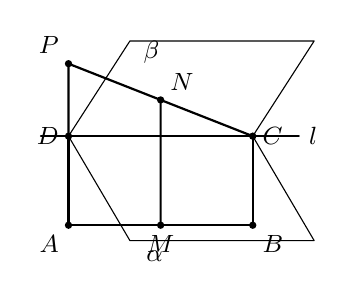
\begin{tikzpicture}[scale=.78,font=\small,line cap=round,line join=round]
  \coordinate (D) at (1,0);
  \coordinate (C) at (4,0);
  \coordinate (A) at (1,-1.45);
  \coordinate (B) at (4,-1.45);
  \coordinate (P) at (1,1.18);
  \coordinate (M) at (2.5,-1.45);
  \coordinate (N) at (2.5,.59);
  % Plane alpha and beta share the line l=DC.
  \draw[thin] (D)--(C)--(5,-1.7)--(2,-1.7)--cycle;
  \draw[thin] (D)--(C)--(5,1.55)--(2,1.55)--cycle;
  \draw[thick] (.55,0)--(4.75,0) node[right] {$l$};
  \node at (2.4,-1.95) {$\alpha$};
  \node at (2.35,1.37) {$\beta$};
  % Rectangle and the given point/segments.
  \draw[thick] (A)--(B)--(C)--(D)--cycle;
  \draw[thick] (P)--(A) (P)--(C) (M)--(N);
  \fill (A) circle (1.7pt) node[below left] {$A$};
  \fill (B) circle (1.7pt) node[below right] {$B$};
  \fill (C) circle (1.7pt) node[right] {$C$};
  \fill (D) circle (1.7pt) node[left] {$D$};
  \fill (P) circle (1.7pt) node[above left] {$P$};
  \fill (M) circle (1.7pt) node[below] {$M$};
  \fill (N) circle (1.7pt) node[above right] {$N$};
\end{tikzpicture}
\end{center}
\nopagebreak[4]
\Needspace{4\baselineskip}
\textbf{解析}
\nopagebreak[4]
\begin{center}% 固定来源 PDF 印刷页 87 第 21 题评分解析辅助构造示意重绘。
% 在原题关系上增加 E 为 DC 中点、Q 为 DP 中点以及连接线；投影不表示度量比例。
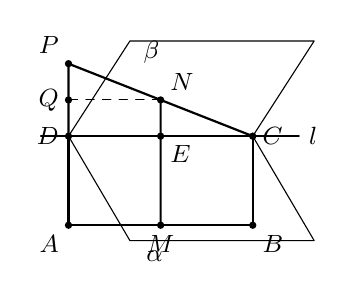
\begin{tikzpicture}[scale=.78,font=\small,line cap=round,line join=round]
  \coordinate (D) at (1,0);
  \coordinate (C) at (4,0);
  \coordinate (A) at (1,-1.45);
  \coordinate (B) at (4,-1.45);
  \coordinate (P) at (1,1.18);
  \coordinate (M) at (2.5,-1.45);
  \coordinate (N) at (2.5,.59);
  \coordinate (E) at (2.5,0);
  \coordinate (Q) at (1,.59);
  \draw[thin] (D)--(C)--(5,-1.7)--(2,-1.7)--cycle;
  \draw[thin] (D)--(C)--(5,1.55)--(2,1.55)--cycle;
  \draw[thick] (.55,0)--(4.75,0) node[right] {$l$};
  \node at (2.4,-1.95) {$\alpha$};
  \node at (2.35,1.37) {$\beta$};
  \draw[thick] (A)--(B)--(C)--(D)--cycle;
  \draw[thick] (P)--(A) (P)--(C) (M)--(N);
  \draw[dashed] (M)--(E) (N)--(E) (N)--(Q) (A)--(Q);
  \fill (A) circle (1.7pt) node[below left] {$A$};
  \fill (B) circle (1.7pt) node[below right] {$B$};
  \fill (C) circle (1.7pt) node[right] {$C$};
  \fill (D) circle (1.7pt) node[left] {$D$};
  \fill (P) circle (1.7pt) node[above left] {$P$};
  \fill (M) circle (1.7pt) node[below] {$M$};
  \fill (N) circle (1.7pt) node[above right] {$N$};
  \fill (E) circle (1.7pt) node[below right] {$E$};
  \fill (Q) circle (1.7pt) node[left] {$Q$};
\end{tikzpicture}
\end{center}
\nopagebreak[4]
\gksubpart{(1) 二面角}

连接 $PD$。由 $PA\perp\alpha$，得 $PA\perp AD$；由矩形 $ABCD$ 及 $AB\parallel l$，得 $AD\perp l$。因此 $PD\perp l$，$\angle PDA$ 是二面角 $\alpha-l-\beta$ 的平面角。

在直角三角形 $PAD$ 中，$PA=AD$，故 $\angle PDA=45^\circ$，即二面角 $\alpha-l-\beta$ 的大小为 $45^\circ$。

\gksubpart{(2) 证明 $MN\perp AB$}

设 $E$ 是 $DC$ 的中点，连接 $ME,NE$。$M,N,E$ 依次是 $AB,PC,DC$ 的中点，故 $ME\parallel AD$，$NE\parallel PD$。于是 $ME\perp l$、$NE\perp l$，从而 $l\perp$ 平面 $MNE$。

又 $AB\parallel l$，故 $AB\perp$ 平面 $MNE$。由于 $MN\subset$ 平面 $MNE$，所以 $MN\perp AB$。

\gksubpart{(3) 异面直线所成角}

设 $Q$ 是 $DP$ 的中点，连接 $NQ,AQ$。由于 $N,Q$ 分别是 $PC,PD$ 的中点，得 $NQ\parallel DC$，且 $NQ=\dfrac12DC$。又 $AM\parallel DC$，且 $AM=\dfrac12AB=\dfrac12DC$，所以 $QN\parallel AM$ 且 $QN=AM$。因此四边形 $QNMA$ 为平行四边形，$AQ\parallel MN$。

于是 $\angle PAQ$ 是异面直线 $PA$ 与 $MN$ 所成的角。在等腰直角三角形 $PAD$ 中，$AQ$ 是斜边 $PD$ 上的中线，故 $\angle PAQ=45^\circ$。

\gkanswer{答案（1）：$45^\circ$}

\gkanswer{答案（2）：$MN\perp AB$}

\gkanswer{答案（3）：$45^\circ$}

\end{answer}
\begin{answer}
\gksolhead{22}{}

\textbf{题目}：

\Needspace{5\baselineskip}
（本题满分 16 分）本题有 A2、B2 两种选做版本。A2 组本题共有 3 个小题，第 1、3 小题各满分 6 分，第 2 小题满分 4 分。设

\nopagebreak[4]
\[
z=a+bi\quad(a,b\in\mathbb R,\ b\ne0,\ i\text{ \text{为虚数单位}}),\qquad w=z+\dfrac1z
\]

是实数，且 $-1<w<2$。

（1） 求 $|z|$ 的值及 $z$ 的实部的取值范围；

（2） 设 $u=\dfrac{1-z}{1+z}$，求证：$u$ 为纯虚数；

（3） 求 $w-u^2$ 的最小值。

\textbf{B2 组：} 本题共有 3 个小题，第 1 小题满分 4 分，第 2 小题满分 5 分，第 3 小题满分 7 分。已知 $A(-1,2)$ 为抛物线 $C:y=2x^2$ 上的点，直线 $l_1$ 过点 $A$，且与抛物线 $C$ 相切。直线 $l_2:x=a\ (a\ne-1)$ 交抛物线 $C$ 于点 $B$，交直线 $l_1$ 于点 $D$。

（1） 求直线 $l_1$ 的方程；

（2） 设 $\triangle ABD$ 的面积为 $S_1$，求 $|BD|$ 及 $S_1$ 的值；

（3） 设由抛物线 $C$、直线 $l_1,l_2$ 所围成的图形的面积为 $S_2$，求证：$S_1:S_2$ 的值为与 $a$ 无关的常数。

\Needspace{4\baselineskip}
\textbf{解析}

\gksubpart{(1) 模长与实部范围（A2 组）}

\nopagebreak[4]
\[
w=a+bi+\dfrac1{a+bi}
=\left(a+\dfrac{a}{a^2+b^2}\right)
+\left(b-\dfrac{b}{a^2+b^2}\right)i.
\]

\Needspace{5\baselineskip}
因为 $w$ 是实数且 $b\ne0$，所以 $a^2+b^2=1$，即 $|z|=1$。于是 $w=2a$；由 $-1<w<2$，得

\nopagebreak[4]
\[
-\dfrac12<a<1.
\]

\gksubpart{(2) 纯虚数与距离、面积（A2/B2 组）}

\Needspace{5\baselineskip}
\textbf{A2 组：}

\nopagebreak[4]
\[
u=\dfrac{1-z}{1+z}
=\dfrac{1-a-bi}{1+a+bi}
=\dfrac{(1-a-bi)(1+a-bi)}{(1+a+bi)(1+a-bi)}
=-\dfrac{b}{a+1}i.
\]

由于 $a\in(-\dfrac12,1)$ 且 $b\ne0$，所以 $u$ 为纯虚数。

\Needspace{5\baselineskip}
\textbf{B2 组：} 抛物线 $y=2x^2$ 在 $A(-1,2)$ 处的切线斜率为 $y'=4x=-4$，所以

\nopagebreak[4]
\[
l_1:y-2=-4(x+1),\qquad 4x+y+2=0.
\]

\Needspace{5\baselineskip}
由 $y=2x^2$ 及 $x=a$，得 $B=(a,2a^2)$；由 $4x+y+2=0$ 及 $x=a$，得 $D=(a,-4a-2)$。所以

\nopagebreak[4]
\[
|BD|=2a^2+4a+2=2(a+1)^2.
\]

\Needspace{5\baselineskip}
点 $A$ 到直线 $BD$ 的距离为 $|a+1|$，从而

\nopagebreak[4]
\[
S_1=\dfrac12|BD|\,|a+1|=|a+1|^3.
\]

\gksubpart{(3) 最小值与面积比（A2/B2 组）}

\Needspace{5\baselineskip}
\textbf{A2 组：} 由 $a^2+b^2=1$ 及 $u=-\dfrac{b}{a+1}i$，

\nopagebreak[4]
\[
\begin{aligned}
w-u^2
&=2a+\dfrac{b^2}{(a+1)^2}\\
&=2a+\dfrac{1-a^2}{(a+1)^2}\\
&=2a+\dfrac{1-a}{a+1}\\
&=2\left[(a+1)+\dfrac1{a+1}\right]-3.
\end{aligned}
\]

因为 $a+1>0$，故 $(a+1)+\dfrac1{a+1}\ge2$，所以 $w-u^2\ge1$。当 $a+1=\dfrac1{a+1}$，即 $a=0$ 时取等号，最小值为 $1$。

\Needspace{5\baselineskip}
\textbf{B2 组：} 当 $a>-1$ 时，

\nopagebreak[4]
\[
S_2=\int_{-1}^{a}(2x^2+4x+2)\,dx=\dfrac23(a+1)^3;
\]

\Needspace{5\baselineskip}
当 $a<-1$ 时，

\nopagebreak[4]
\[
S_2=\int_{a}^{-1}(2x^2+4x+2)\,dx=-\dfrac23(a+1)^3.
\]

\Needspace{5\baselineskip}
因此 $S_2=\dfrac23|a+1|^3$，从而

\nopagebreak[4]
\[
S_1:S_2=\dfrac32:1=3:2,
\]

该比值与 $a$ 无关。

\gkanswer{答案（1）：A2 组 $|z|=1$，$\operatorname{Re}z\in(-\dfrac12,1)$；B2 组 $l_1:4x+y+2=0$。}

\gkanswer{答案（2）：A2 组 $u$ 为纯虚数；B2 组 $|BD|=2(a+1)^2$，$S_1=|a+1|^3$。}

\gkanswer{答案（3）：A2 组最小值为 $1$；B2 组 $S_1:S_2=3:2$。}

\end{answer}
\begin{answer}
\gksolhead{23}{}

\textbf{题目}：

（本题满分 18 分）第 1、2 小题各满分 4 分，第 3 小题满分 10 分。已知双曲线 $S$ 的两条渐近线过坐标原点，且与以点 $A(\sqrt2,0)$ 为圆心、$1$ 为半径的圆相切；双曲线 $S$ 的一个顶点 $A'$ 与点 $A$ 关于直线 $y=x$ 对称。

（1） 求双曲线 $S$ 的方程；

（2） 设直线 $l$ 过点 $A$，斜率为 $1$。在双曲线 $S$ 的上支上求点 $B$，使其与直线 $l$ 的距离为 $\sqrt2$；

（3） 求双曲线 $S$ 上到直线 $l:y=\dfrac{2\sqrt5}{5}(x-\sqrt2)$ 的距离为 $\sqrt2$ 的点的个数。
\nopagebreak[4]
\begin{center}% 固定来源 PDF 印刷页 86 第 23 题双曲线、渐近线及圆的结构示意重绘。
% 双曲线、圆心 A、圆半径和渐近线按题面关系作图；示意不添加未给定条件。
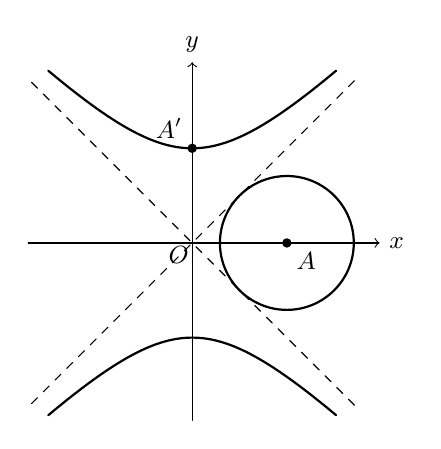
\begin{tikzpicture}[x=.85cm,y=.85cm,font=\small,line cap=round,line join=round]
  \draw[->] (-2.45,0)--(2.8,0) node[right] {$x$};
  \draw[->] (0,-2.65)--(0,2.7) node[above] {$y$};
  \draw[dashed] (-2.4,-2.4)--(2.5,2.5);
  \draw[dashed] (-2.4,2.4)--(2.5,-2.5);
  \draw[thick,domain=-2.15:2.15,samples=100,variable=\x]
    plot (\x,{sqrt(\x*\x+2)});
  \draw[thick,domain=-2.15:2.15,samples=100,variable=\x]
    plot (\x,{-sqrt(\x*\x+2)});
  \draw[thick] (1.4142,0) circle (1);
  \fill (0,1.4142) circle (1.7pt) node[above left] {$A'$};
  \fill (1.4142,0) circle (1.7pt) node[below right] {$A$};
  \node[below left,inner sep=1pt] at (0,0) {$O$};
\end{tikzpicture}
\end{center}
\nopagebreak[4]
\Needspace{4\baselineskip}
\textbf{解析}

\gksubpart{(1) 双曲线方程}

\Needspace{5\baselineskip}
已知双曲线的渐近线为 $y=\pm x$，故其为等轴双曲线。一个顶点为 $A'(0,\sqrt2)$，所以

\nopagebreak[4]
\[
\dfrac{y^2}{2}-\dfrac{x^2}{2}=1.
\]

\gksubpart{(2) 求点 $B$}

\Needspace{5\baselineskip}
设 $B=(x,\sqrt{x^2+2})$。直线 $l$ 为 $y=x-\sqrt2$。点 $B$ 到 $l$ 的距离为 $\sqrt2$，故

\nopagebreak[4]
\[
\dfrac{|x-\sqrt{x^2+2}-\sqrt2|}{\sqrt2}=\sqrt2.
\]

解得 $x=\sqrt2$，$y=2$，故 $B=(\sqrt2,2)$。

\gksubpart{(3) 点的个数}

\Needspace{5\baselineskip}
设直线 $l':y=\dfrac{2\sqrt5}{5}x+m$ 与 $l$ 平行，且两线间的距离为 $\sqrt2$。由点 $A(\sqrt2,0)$ 到 $l'$ 的距离为 $\sqrt2$，

\nopagebreak[4]
\[
\dfrac{|\dfrac{2\sqrt{10}}5+m|}{\dfrac{3\sqrt5}5}=\sqrt2,
\]

\Needspace{5\baselineskip}
解得 $m_1=\dfrac{\sqrt{10}}5$，$m_2=-\sqrt{10}$。对应直线为

\nopagebreak[4]
\[
l_1:y=\dfrac{2\sqrt5}{5}x+\dfrac{\sqrt{10}}5,
\qquad l_2:y=\dfrac{2\sqrt5}{5}x-\sqrt{10}.
\]

\Needspace{5\baselineskip}
将 $l_1$ 代入 $y^2-x^2=2$，得

\nopagebreak[4]
\[
x^2-4\sqrt2x+8=0,
\]

\Needspace{5\baselineskip}
其判别式为 $0$，故 $l_1$ 与双曲线只有一个公共点。将 $l_2$ 代入，得

\nopagebreak[4]
\[
x^2+20\sqrt2x-40=0,
\]

其判别式为 $960>0$，故 $l_2$ 与双曲线有两个公共点。因此所求点数为 $1+2=3$。

\gkanswer{答案（1）：$\dfrac{y^2}{2}-\dfrac{x^2}{2}=1$}

\gkanswer{答案（2）：$B=(\sqrt2,2)$}

\gkanswer{答案（3）：$3$ 个}

\end{answer}
\begin{answer}
\gksolhead{24}{}

\textbf{题目}：

\Needspace{5\baselineskip}
（本题满分 18 分）本题共有 2 个小题，第 1 小题满分 6 分，第 2 小题满分 12 分。设 $A_n$ 为数列 $\{a_n\}$ 的前 $n$ 项和，

\nopagebreak[4]
\[
A_n=\dfrac{3}{2}(a_n-1)\quad(n\in\mathbb N),
\]

\Needspace{5\baselineskip}
数列 $\{b_n\}$ 的通项公式为

\nopagebreak[4]
\[
b_n=4n+3\quad(n\in\mathbb N)\text{。}
\]

（1） 求数列 $\{a_n\}$ 的通项公式；

（2） 若 $d\in\{a_1,a_2,a_3,\ldots\}\cap\{b_1,b_2,b_3,\ldots\}$，则称 $d$ 为数列 $\{a_n\}$ 与 $\{b_n\}$ 的公共项。将这两个数列的公共项按它们在原数列中的先后顺序排成一个新数列 $\{d_n\}$，证明数列 $\{d_n\}$ 的通项公式为 $d_n=3^{2n+1}\ (n\in\mathbb N)$。

\Needspace{4\baselineskip}
\textbf{解析}

\gksubpart{(1) 数列 $\{a_n\}$ 的通项}

\Needspace{5\baselineskip}
当 $n=1$ 时，$A_1=a_1=\dfrac32(a_1-1)$，解得 $a_1=3$。当 $n\ge2$ 时，

\nopagebreak[4]
\[
a_n=A_n-A_{n-1}=\dfrac32(a_n-a_{n-1}),
\]

\Needspace{5\baselineskip}
所以 $a_n=3a_{n-1}$。故 $\{a_n\}$ 是首项为 $3$、公比为 $3$ 的等比数列，

\nopagebreak[4]
\[
a_n=3^n\quad(n\in\mathbb N).
\]

\gksubpart{(2) 公共项数列}

\textbf{证明一：}

\Needspace{5\baselineskip}
（i）先证明形如 $3^{2n+1}\ (n\in\mathbb N)$ 的数是两个数列的公共项。由于 $a_n=3^n$，有 $3^{2n+1}\in\{a_1,a_2,\ldots\}$。又

\nopagebreak[4]
\[
3^{2n+1}=3\cdot9^n=3(8+1)^n=3(8t+1)=4(6t)+3,
\]

其中 $t$ 为正整数，故 $3^{2n+1}$ 也是数列 $\{b_n\}$ 的项。

\Needspace{5\baselineskip}
（ii）再证明数列 $\{a_n\}$ 中其余项都不是 $\{b_n\}$ 的项。$a_1=3$ 不是 $\{b_n\}$ 的项；而

\nopagebreak[4]
\[
a_{2n}=3^{2n}=(8+1)^n=8t+1=4(2t)+1
\]

不可能是 $4m+3$ 的形式，因此不是 $\{b_n\}$ 的项。由（i）、（ii），公共项依次为 $a_3,a_5,a_7,\ldots$，所以 $d_n=a_{2n+1}=3^{2n+1}$。

\textbf{证明二：}

\Needspace{5\baselineskip}
由计算可知，$a_1,a_2$ 不是数列 $\{b_n\}$ 中的项，而 $a_3=27=4\times6+3$，是数列 $\{b_n\}$ 的第 6 项。设 $a_k=3^k$ 是数列 $\{b_n\}$ 的第 $m$ 项，即

\nopagebreak[4]
\[
3^k=4m+3\quad(k,m\in\mathbb N).
\]

\Needspace{5\baselineskip}
则

\nopagebreak[4]
\[
a_{k+1}=3^{k+1}=3(4m+3)=4(3m+2)+1,
\]

\Needspace{5\baselineskip}
不是数列 $\{b_n\}$ 中的项；而

\nopagebreak[4]
\[
a_{k+2}=3^{k+2}=9(4m+3)=4(9m+6)+3
\]

\Needspace{5\baselineskip}
是数列 $\{b_n\}$ 中的项。故公共项依次为 $a_3,a_5,a_7,\ldots$，即

\nopagebreak[4]
\[
d_n=a_{2n+1}=3^{2n+1}\quad(n\in\mathbb N).
\]

\gkanswer{答案（1）：$a_n=3^n$}

\gkanswer{答案（2）：$d_n=3^{2n+1}$}

\end{answer}